%%%%%%%%%%%%%%%%%%%%%%%%%%%%%%%%%%%%%%%%%%%%%%%%%%%%%%%%%%%%%%%%%%%%%%%%%%%%%%%
%%                                                                           %%
%%   Dr Derek Harter                                                         %%
%%   Profesor, Department of Computer Science                                %% 
%%   Texas A&M University - Commerce, USA                                    %%
%%                                                                           %%
%%%%%%%%%%%%%%%%%%%%%%%%%%%%%%%%%%%%%%%%%%%%%%%%%%%%%%%%%%%%%%%%%%%%%%%%%%%%%%%
%%%%     SETTING STARTS - DO NOT CHANGE Unless your TeX setting require so   %%
%%%%%%%%%%%%%%%%%%%%%%%%%%%%%%%%%%%%%%%%%%%%%%%%%%%%%%%%%%%%%%%%%%%%%%%%%%%%%%%
%%----------------------------------------------------------------------------------
% DO NOT Change this. It is the required setting letterpaper page, 11pt, onside print, book style
%%----------------------------------------------------------------------------------
\documentclass[letterpaper,11pt,oneside]{book}

%%-------------------------------------
%% Page margin settings - % half inch margin all sides (recommended)
%%-------------------------------------
\usepackage[margin=1.2in]{geometry} 

%%-------------------------------------
%% Font settings - % CM San or Ariel (recommended)
%%-------------------------------------
% Switch the following two line off: to revert back to default LaTex font (NOT recommended)
\usepackage{amsfonts}
\renewcommand*\familydefault{\sfdefault}

%%-------------------------------------
%% Math/Definition/Theorem/Algorithm packages settings 
%%-------------------------------------
\usepackage[cmex10]{amsmath}
\usepackage{amssymb}
\usepackage{amsthm}
\newtheorem{mydef}{Definition}
\newtheorem{mytherm}{Theorem}

%%-------------------------------------
%% Algorithms/Code Listing environment settings  - 
%% Please do not change these settings
%%-------------------------------------
\usepackage{algorithm}
\usepackage{algpseudocode}
\renewcommand{\algorithmicrequire}{\textbf{Input:}}
\renewcommand{\algorithmicensure}{\textbf{Output:}}
\usepackage[utf8]{inputenc}
\usepackage{listings}
\usepackage{xcolor}
\definecolor{codegreen}{rgb}{0,0.6,0.1}
\definecolor{codegray}{rgb}{0.5,0.5,0.5}
\definecolor{codeblue}{rgb}{0.10,0.00,1.00}
\definecolor{codepurple}{rgb}{0.58,0,0.82}
\definecolor{backcolour}{rgb}{1.0,1.0,1.0}

\lstdefinestyle{mystyle}{
    backgroundcolor=\color{backcolour},   
    commentstyle=\color{codegreen},
    keywordstyle=\color{codeblue},
    numberstyle=\tiny\color{codegray},
    stringstyle=\color{codepurple},
    basicstyle=\ttfamily\footnotesize,
    breakatwhitespace=false,         
    breaklines=true,                 
    captionpos=b,                        
    keepspaces=true,                 
    numbers=left,                    
    numbersep=5pt,                  
    showspaces=false,                
    showstringspaces=false,
    showtabs=false,                  
    tabsize=2,
    frame=none
}
\lstset{style=mystyle}

%%-------------------------------------
%% Graphics/Figures environment settings
%%-------------------------------------
\usepackage{graphicx}
\usepackage{subfigure}
\usepackage{caption}
\usepackage{lipsum}

%%-------------------------------------
%% Table environment settings
%%-------------------------------------
\usepackage{multirow}
\usepackage{rotating}
\usepackage{makecell}
\usepackage{booktabs}
%\usepackage{longtable,booktabs}

%%-------------------------------------
%% List of Abbreviations settings
%%-------------------------------------
\usepackage{enumitem}
\newlist{abbrv}{itemize}{1}
\setlist[abbrv,1]{label=,labelwidth=1in,align=parleft,itemsep=0.1\baselineskip,leftmargin=!}

%%-------------------------------------
%% Bibliography/References settings   - Harvard Style was used in this report
%%-------------------------------------
\usepackage[hidelinks]{hyperref}
\usepackage[comma,authoryear]{natbib}
\renewcommand{\bibname}{References} % DO NOT remove or switch of 

%%-------------------------------------
%% Appendix settings     
%%-------------------------------------
\usepackage[toc]{appendix}
%%%%%%%%%%%%%%%%%%%%%%%%%%%%%%%%%%%%%%%%%%%%%%%%%%%%%%%%%%%%%%%%%%%%%%%%%%%%%%%%%%%%%%%
%%%%                     SETTING ENDS                                            %%%%%%
%%%%%%%%%%%%%%%%%%%%%%%%%%%%%%%%%%%%%%%%%%%%%%%%%%%%%%%%%%%%%%%%%%%%%%%%%%%%%%%%%%%%%%%
\begin{document}

    \captionsetup[figure]{margin=1.5cm,font=small,name={Figure},labelsep=colon}
    \captionsetup[table]{margin=1.5cm,font=small,name={Table},labelsep=colon}
    \SetLipsumDefault{1}
    
    \frontmatter
    
    \begin{titlepage}      
        \begin{center}
            
\includegraphics[width=3cm]{figures/tamuc-logo.png}\\[0.5cm]
            {\LARGE Texas A\&M University - Commerce\\[0.5cm]
            Department of Computer Science}\\[2cm]
			%{\color{blue} \rule{\textwidth}{1pt}}
			
			% -------------------------------
			% You need to edit some details here
			% -------------------------------  
            \linespread{1.2}\huge {
                %%%%%%%%%%%%%%%%%%%%%%%%%%%%
                %TODO: 1 TITLE of Your PROJECT 
                %%%%%%%%%%%%%%%%%%%%%%%%%%%%
                % chnage the following line                
                VeracityVigil: Unmasking Deception through Advanced NLP Analysis 
            
            }
            \linespread{1}~\\[2cm]
			%{\color{blue} \rule{\textwidth}{1pt}}
            {\Large 
                %%%%%%%%%%%%%%%%%%%%%%%%%%%%
                %TODO: 2 YOUR NAME
                %%%%%%%%%%%%%%%%%%%%%%%%%%%%             
                % chnage the following line
                Najeebuddin Mohammed
                % change end             
            }\\[1cm] 
            

            {\large 
                %%%%%%%%%%%%%%%%%%%%%%%%%%%%
                %TODO: 3 YOUR NAME Supervisor's name(s)
                %%%%%%%%%%%%%%%%%%%%%%%%%%%%             
                % change the following line                
                \emph{Supervisor:} Derek Harter, Ph.D.}\\[1cm] % if applicable
            
    		% PLEASE DO NOT CHANGE THIS TEXT %
            \large A report submitted in partial fulfilment of the requirements of\\Texas A\&M University - Commerce for the degree of\\ Master of Science in \textit{Computer Science}\\[0.3cm] 
            \vfill
            
            
            \today % Please update this date you can use \date{April 2020} for fixed date
        \end{center}
    \end{titlepage}
    
    
    % -------------------------------------------------------------------
    % Declaration
    % -------------------------------------------------------------------
    \newpage
    \thispagestyle{empty}
    \chapter*{\Large Declaration}
    % PLEASE CHANGE THIS TEXT EXCEPT YOUR NAME%
    % -------------------------------
    %TODO: PLEASE ONLY UPDATE HERE -- PLEASE WRITE YOUR NAME %    
    % ------------------------------- 
    I,
    %%%%%%%%%%%%%%%%%%%%%%%
     Najeebuddin Mohammed, % Mandatory part
    %%%%%%%%%%%%%%%%%%%%%%%
    of the Department of Computer Science, Texas A\&M University - Commerce, confirm that this is my own work and figures, tables, equations, code snippets, artworks, and illustrations in this report are original and have not been taken from any other person's work, except where the works of others have been explicitly acknowledged, quoted, and referenced. I understand that if failing to do so will be considered a case of plagiarism. Plagiarism is a form of academic misconduct and will be penalised accordingly. \\
    
    %% Please delete as appropriate. 
    \noindent
    %%%%%%%%%%%%%%%%%%%%%%%%%%%%%%%%%%%%%%%%%%%%%%% 
    %TODO 1 Consent for example copy -  we will use 
    I give consent to a copy of my report being shared with future students as an exemplar. \\
    
    \noindent
    %%%%%%%%%%%%%%%%%%%%%%%%%%%%%%%%%%%%%%%%%%%%%%% 
    %TODO 2 Consent to let the report to use use by library for public use
    I give consent for my work to be made available more widely to members of TAMUC and public with interest in teaching, learning and research. 
    %%%%%%%%%%%%%%%%%%%%%%%%%%%%%%%%%%%%%%%%%%%%%%%
    ~\\[1cm]
    \begin{flushright}
	%------------------------------ 
	% change the following line
    %TODO: PLEASE UPDATE  Your Name  -------------------------------%
	Najeebuddin Mohammed % Please change it to your name
    
    \today
    \end{flushright}

     
    % -------------------------------------------------------------------
    % Abstract and Acknowledgement
    % -------------------------------------------------------------------
    
    %Two resources useful for abstract writing.
% Guidance of how to write an abstract/summary provided by Nature: https://cbs.umn.edu/sites/cbs.umn.edu/files/public/downloads/Annotated_Nature_abstract.pdf %https://writingcenter.gmu.edu/guides/writing-an-abstract
\chapter*{\center \Large  Abstract}
%%%%%%%%%%%%%%%%%%%%%%%%%%%%%%%%%%%%%%
% Replace all text with your text
%%%%%%%%%%%%%%%%%%%%%%%%%%%%%%%%%%%

This is a graduate project report template and instruction on how to write a report. It also has some useful examples to use \LaTeX. Do read this template carefully. The number of chapters and their titles may vary depending on the type of project and personal preference. Section titles in this template are illustrative and should be updated accordingly. For example, sections named ``A section...'' and ``Example of ...'' should be updated. The number of sections in each chapter may also vary. This template may or may not suit your project. Discuss the structure of your report with your supervisor.

%%%
~\\[1cm]%REMOVE THIS
\noindent\textbf{Guidance on abstract writing:} An abstract is a summary of a report in a single paragraph up to a maximum of 250 words. An abstract should be self-contained, and it should not refer to sections, figures, tables, equations, or references. An abstract typically consists of sentences describing the following four parts: (1) introduction (background and purpose of the project), (2) methods, (3) results and analysis, and (4) conclusions. The distribution of these four parts of the abstract should reflect the relative proportion of these parts in the report itself. An abstract starts with a few sentences describing the project's general field, comprehensive background and context, the main purpose of the project; and the problem statement. A few sentences describe the methods, experiments, and implementation of the project. A few sentences describe the main results achieved and their significance. The final part of the abstract describes the conclusions and the implications of the results to the relevant field.


%%%%%%%%%%%%%%%%%%%%%%%%%%%%%%%%%%%%%%%%%%%%%%%%%%%%%%%%%%%%%%%%%%%%%%%%%s
~\\[1cm]
\noindent % Provide your key words
\textbf{Keywords:} a maximum of five keywords/keyphrase separated by commas

\vfill
\noindent
\textbf{Report's total word count:} we expect a maximum of 10,000 words (excluding reference and appendices) and about 10 pages. [A good project report can also be written in approximately 5,000 words.]


    % -------------------------------------------------------------------
	% Acknowledgement
	% -------------------------------------------------------------------
   
    \chapter*{\center \Large  Acknowledgements}
%%%% Update with your text %%%%%%%%%%%%%%%
An acknowledgements section is optional. You may like to acknowledge the support and help of your supervisor(s), friends, or any other person(s), department(s), institute(s), etc. If you have been provided specific facility from department/school acknowledged so.  

   
    
    % -------------------------------------------------------------------
    % Contents, list of figures, list of tables
    % -------------------------------------------------------------------
    
    \tableofcontents
    \listoffigures
    \listoftables
    \chapter*{List of Abbreviations}
\chaptermark{List of Abbreviations}
%%%%%%%%%%%%%%%%%%%%%%%%%%%%%%%%%%%
%%  Enter your list of Abbreviation and Symbols in this file
%%%%%%%%%%%%%%%%%%%%%%%%%%%%%%%%%%%
\begin{abbrv}
    
    \item[SMPCS]			School of Mathematical, Physical and Computational Sciences
    
\end{abbrv}
 %  Enter your list of Abbreviation and Symbols in this file
    
    %%%%%%%%%%%%%%%%%%%%%%%%%%%%%%%%%%%%%%%%%%%%%%%%%%%%%%%%%%%%%%%%%%%%%%%%
    %%                                                                    %%  
    %%  Main chapters and sections of your project                        %%  
    %%  Everything from here on needs updates in your own words and works %%
    %%                                                                    %%
    %%%%%%%%%%%%%%%%%%%%%%%%%%%%%%%%%%%%%%%%%%%%%%%%%%%%%%%%%%%%%%%%%%%%%%%%
    \mainmatter
    % Read for preparation of document in LaTex 
    % Lamport, L. (1986), LATEX: A Document Preparation System, Addison-Wesley.
    
    \chapter{Introduction}
\label{ch:into} % This how you label a chapter and the key (e.g., ch:into) will be used to refer this chapter ``Introduction'' later in the report. 
% the key ``ch:into'' can be used with command \ref{ch:intor} to refere this Chapter.



%%%%%%%%%%%%%%%%%%%%%%%%%%%%%%%%%%%%%%%%%%%%%%%%%%%%%%%%%%%%%%%%%%%%%%%%%%%%%%%%%%%
\section{Background}
\label{sec:into_back}
The pervasive dissemination of misinformation in online articles presents a critical challenge 
in today's information landscape. This project delves into the intersection of Natural Language 
Processing (NLP) and machine learning to address this issue. Motivated by the increasing impact 
of fake news on public perception and decision-making, the project seeks to contribute to the 
development of robust mechanisms for detecting and mitigating the spread of deceptive content. 

%%%%%%%%%%%%%%%%%%%%%%%%%%%%%%%%%%%%%%%%%%%%%%%%%%%%%%%%%%%%%%%%%%%%%%%%%%%%%%%%%%%
\section{Problem statement}
\label{sec:intro_prob_art}
Despite advancements in fake news detection techniques, accurately identifying deceptive content in online articles remains a significant challenge. Traditional machine learning approaches often struggle to capture the nuanced linguistic patterns and contextual information present in text data, leading to suboptimal performance in distinguishing between real and fake news articles. Therefore, there is a need to explore more sophisticated methods, such as LSTM networks, to improve the accuracy and effectiveness of fake news detection. The  dataset utilized in this research, referred to as the ISOT Fake News \cite{fake-news}

%%%%%%%%%%%%%%%%%%%%%%%%%%%%%%%%%%%%%%%%%%%%%%%%%%%%%%%%%%%%%%%%%%%%%%%%%%%%%%%%%%%
\section{Aims and objectives}
\label{sec:intro_aims_obj}
\textbf{Aims:} To enhance the precision of fake news detection within a corpus of news articles in \cite{fake-news} using LSTM networks. 

\textbf{Objectives:} 
\begin{enumerate}
    \item Evaluate the effectiveness of LSTM networks in discerning distinctive linguistic patterns associated with fake news sources within the defined news article corpus.\citep{fake-news} 
    \item Investigate the impact of LSTM-based models on improving the accuracy of fake news detection compared to traditional machine learning approaches. 
    \item Explore techniques for optimizing LSTM architectures, including hyperparameter tuning and model regularization, to achieve better performance in fake news classification tasks. 
\end{enumerate}
 



%%%%%%%%%%%%%%%%%%%%%%%%%%%%%%%%%%%%%%%%%%%%%%%%%%%%%%%%%%%%%%%%%%%%%%%%%%%%%%%%%%%
\section{Solution approach}
\label{sec:intro_sol} % label of Org section
The solution approach involves leveraging LSTM networks as the primary technique for fake news detection in online articles. The methodology includes the following steps:

\subsection{Dataset Description}

The dataset utilized in this study, known as the ISOT Fake News Dataset (2018), contains a collection of news articles with associated labels indicating whether each article is real or fake. The dataset comprises X instances with Y attributes, including features such as 'Title', 'Text', and 'Label'. 'Label' indicates whether an article is classified as real or fake news.

\subsection{Data Preprocessing}

Data preprocessing plays a crucial role in preparing the dataset for analysis. In this phase, several steps are undertaken:

\subsubsection{Text Cleaning}Removal of special characters, punctuation, and irrelevant symbols to ensure uniformity in the textual data.
\subsubsection{Tokenization}
 Breaking down the text into individual tokens or words to facilitate further processing.
\subsubsection{Stopword Removal}
 Elimination of common words such as 'the', 'and', and 'is' that do not contribute significantly to the classification task.
\subsubsection{Vectorization}
 Conversion of text data into numerical vectors using techniques like TF-IDF or word embeddings.
\subsection{Model Implementation}

Following data preprocessing, the primary focus is on implementing machine learning models, particularly LSTM networks, for fake news detection. The steps involved in model implementation are as follows:

\subsubsection{Architecture Design}
 Designing LSTM-based deep learning models for binary classification of news articles into real or fake categories.
\subsubsection{Training}
 Training the LSTM models using the preprocessed dataset and optimizing the model parameters for improved performance.
\subsubsection{Evaluation}
 Assessing the trained models' performance using standard evaluation metrics such as accuracy, precision, recall, and F1-score.
\subsection{Performance Analysis}

To optimize the LSTM models' performance, hyperparameter tuning is conducted using techniques such as grid search or random search. The hyperparameters under consideration may include the number of LSTM units, learning rate, dropout rate, and batch size. Performance analysis involves comparing the LSTM models' performance against baseline models and traditional machine learning algorithms, highlighting the LSTM networks' effectiveness in fake news detection.
 

%%%%%%%%%%%%%%%%%%%%%%%%%%%%%%%%%%%%%%%%%%%%%%%%%%%%%%%%%%%%%%%%%%%%%%%%%%%%%%%%%%%
\section{Summary of contributions and achievements}
In our research on fake news detection, we've contributed significantly to improving the accuracy of identifying deceptive content in online articles. By leveraging advanced techniques like LSTM networks, we've delved deep into the linguistic patterns of fake news and developed models that can better discern between real and deceptive articles. Through systematic experimentation and model optimization, we've demonstrated the effectiveness of LSTM architectures in enhancing fake news detection compared to traditional methods. Our work not only provides insights into the nuances of fake news detection but also offers practical solutions for mitigating the spread of misinformation.

Furthermore, our study extends beyond model implementation to encompass rigorous data preprocessing, hyperparameter tuning, and performance analysis. By meticulously cleaning and preparing the dataset, we ensure the reliability and accuracy of our results. Through techniques like grid search for hyperparameter optimization, we identify the best-performing models and parameters, thereby maximizing the predictive performance of our fake news detection systems. Our comprehensive approach, coupled with clear documentation, contributes to the reproducibility and reliability of our findings, facilitating further advancements in the field of misinformation detection and mitigation.
%  use this section 
\label{sec:intro_sum_results} % label of summary of results



%%%%%%%%%%%%%%%%%%%%%%%%%%%%%%%%%%%%%%%%%%%%%%%%%%%%%%%%%%%%%%%%%%%%%%%%%%%%%%%%%%%

    \chapter{Literature Review}
\label{ch:lit_rev} %Label of the chapter lit rev. The key ``ch:lit_rev'' can be used with command \ref{ch:lit_rev} to refer this Chapter.

The realm of social media, encompassing forums, social networking, microblogging, social 
bookmarking, and wikis \citep{esrc,gil2019}, significantly influences the dynamics of 
information dissemination. However, the unintentional factors contributing to the rise of fake 
news, as evidenced by incidents like the Nepal Earthquake case 
\citep{tandoc2017,radianti2016}, underline the intricacies of navigating the digital 
information landscape. In 2020, the global health sector encountered a substantial surge in 
fake news, prompting the World Health Organization (WHO) to declare an 'infodemic' during the 
COVID-19 outbreak. This infodemic involved a flood of both authentic and false information, 
including a noteworthy volume of misinformation.

In response to the challenges of identifying and combating fake news, several research 
initiatives have proposed innovative solutions. \cite{sahoo2021multiple} introduced an 
automatic fake news identification technique tailored for the Chrome environment, providing a 
means to detect fake news on Facebook. This approach leverages various features associated with 
a Facebook account, coupled with news content features, utilizing deep learning to analyze 
account characteristics.

FakeNewsNet, presented by \cite{shu2020fakenewsnet}, serves as a valuable repository of fake 
news data. This resource provides datasets with diverse features, spatiotemporal information, 
and social context, facilitating research in the domain of fake news. Evaluation indicates that 
user engagements can contribute to fake news detection in addition to news articles, 
highlighting the multifaceted nature of information dissemination.

\cite{Kumar} proposed a CNN and bidirectional LSTM ensembled network for identifying original 
and false news instances. Utilizing various advanced approaches, such as Long Short Term 
Memories LSTMs, Convolutional Neural Networks CNNs, attention mechanisms, and ensemble methods, 
the study collected news instances from sources like PolitiFact. The CNN and bidirectional LSTM 
ensembled network, incorporating an attention mechanism, demonstrated superior accuracy, 
emphasizing the significance of model complexity in addressing the fake news identification 
challenge.

Natural Language Processing (NLP) emerges as a pivotal tool in tackling fake news. 
\cite{choudhary2021linguistic} proposed a linguistic model, employing handcrafted linguistic 
features for fake news detection. The model, driven by language-specific features, demonstrated 
a remarkable 86\% accuracy in detecting and categorizing fake messages. Additionally, 
\cite{abdullah2020fake} adopted a multimodal approach, combining Convolutional Neural Network 
(CNN) and Long Short-Term Memory (LSTM), achieving significant performance in classifying fake 
news articles based on source, history, and linguistic cues.

Furthermore, \cite{aslam2021fake} introduced an ensemble-based deep learning model for 
classifying news as fake or real using the LIAR dataset. Employing a combination of Bi-LSTM-GRU-
dense and dense deep learning models, the study achieved notable accuracy, recall, precision, 
and F-score. Despite these advancements, ongoing research aims to enhance the robustness of 
these models, emphasizing the need for continual improvement and exploration of diverse 
datasets in fake news detection.



% A possible section of you chapter
\section{Evaluation of Existing Scholarship on Fake News Detection } % Use this section title or choose a betterone
The comprehensive examination of the literature reveals a multifaceted landscape in the realm 
of fake news identification. Researchers employ diverse strategies, ranging from linguistic 
models to multimodal approaches, emphasizing the need for a holistic understanding that 
incorporates both content and social context. Key findings underscore the significance of model 
complexity, with advanced architectures like the CNN bidirectional LSTM ensembled network 
exhibiting notable success. Natural Language Processing (NLP) emerges as a critical tool in 
deciphering news content, demonstrated by linguistic models and the utilization of NLP 
techniques for textual attribute analysis. Despite considerable progress, there remains a 
persistent call for improvement, urging researchers to explore feature richness, latent 
semantic features, and diverse datasets. The global impact of infodemics, particularly 
highlighted during the COVID-19 outbreak, underscores the urgency in developing robust fake 
news detection systems. In essence, the literature review illuminates the dynamic and evolving 
nature of fake news research, emphasizing innovation and adaptability in response to the 
challenges presented in the digital information age.
\\

% Pleae use this section
\section{Summary} 
In summary, this literature review provides a comprehensive exploration of the current state of 
research in the field of fake news detection. The chapter commences by delineating the 
landscape of social media and its role in the dissemination of misinformation. It delves into 
the inadvertent factors contributing to the emergence of fake news, exemplifying instances such 
as the Nepal Earthquake case. The review accentuates the gravity of the 'infodemic,' 
particularly evident during the COVID-19 outbreak, necessitating advanced detection mechanisms. 
Several notable research endeavors are scrutinized, including \cite{sahoo2021multiple} automatic fake 
news identification technique, \cite{shu2020fakenewsnet} repository, and \cite{Kumar}
CNN+bidirectional LSTM ensembled network. The significance of Natural Language Processing (NLP) 
in understanding and detecting fake news is highlighted through studies like \cite{choudhary2021linguistic} 
linguistic model. The literature underscores the need for continuous innovation, feature 
exploration, and adaptation to address the evolving challenges posed by the rampant spread of 
fake news. This synthesis of existing knowledge provides a robust foundation for the ensuing 
research endeavors aimed at enhancing the efficacy of fake news detection systems.~\\
% https://guides.library.bloomu.edu/litreview
    % replace all text with your own text.
% in this template few examples are mention
\chapter{Methodology}
\label{ch:method} % Label for method chapter

\subsubsection{Data Collection}

The ISOT Fake News Dataset serves as the foundation for this research endeavor, comprising articles categorized into real and fake news. Through meticulous collection efforts, articles were sourced from reputable platforms like Reuters.com for truthful content and flagged unreliable sources for fake news articles. The dataset's temporal focus on articles primarily from 2016 to 2017 aligns with a period marked by significant political discourse, making it particularly relevant for studying misinformation dynamics.

Consisting of two CSV files, "True.csv" and "Fake.csv," the dataset offers over 12,600 articles each, providing a rich and diverse collection for analysis. Each article within the dataset includes essential information such as the article title, text, publication date, and categorization as real or fake news. By retaining certain characteristics of fake news articles, such as punctuation and mistakes, the dataset aims to authentically reflect the nature of misinformation encountered in real-world contexts, ensuring its relevance and utility for research purposes.

 \begin{figure}

     \centering
     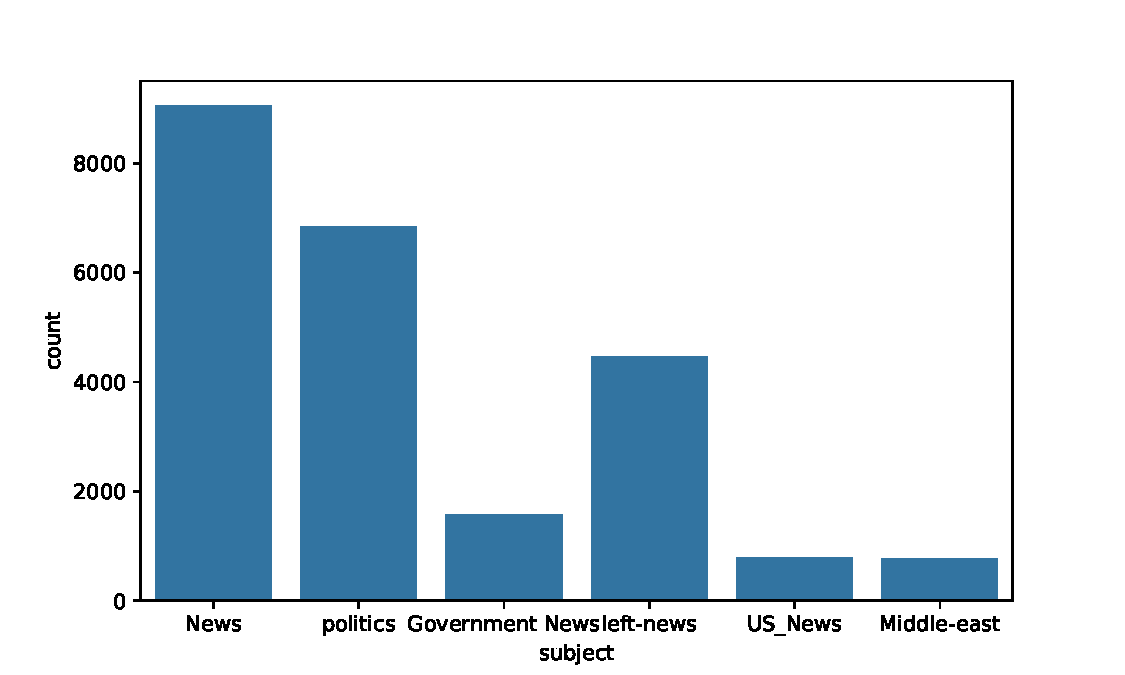
\includegraphics[width=1\linewidth]{figures/FakeNewCategories.pdf}
     \caption{Fake News Categories}
     \label{fig:enter-label}
 \end{figure}

\begin{figure}
    \centering
    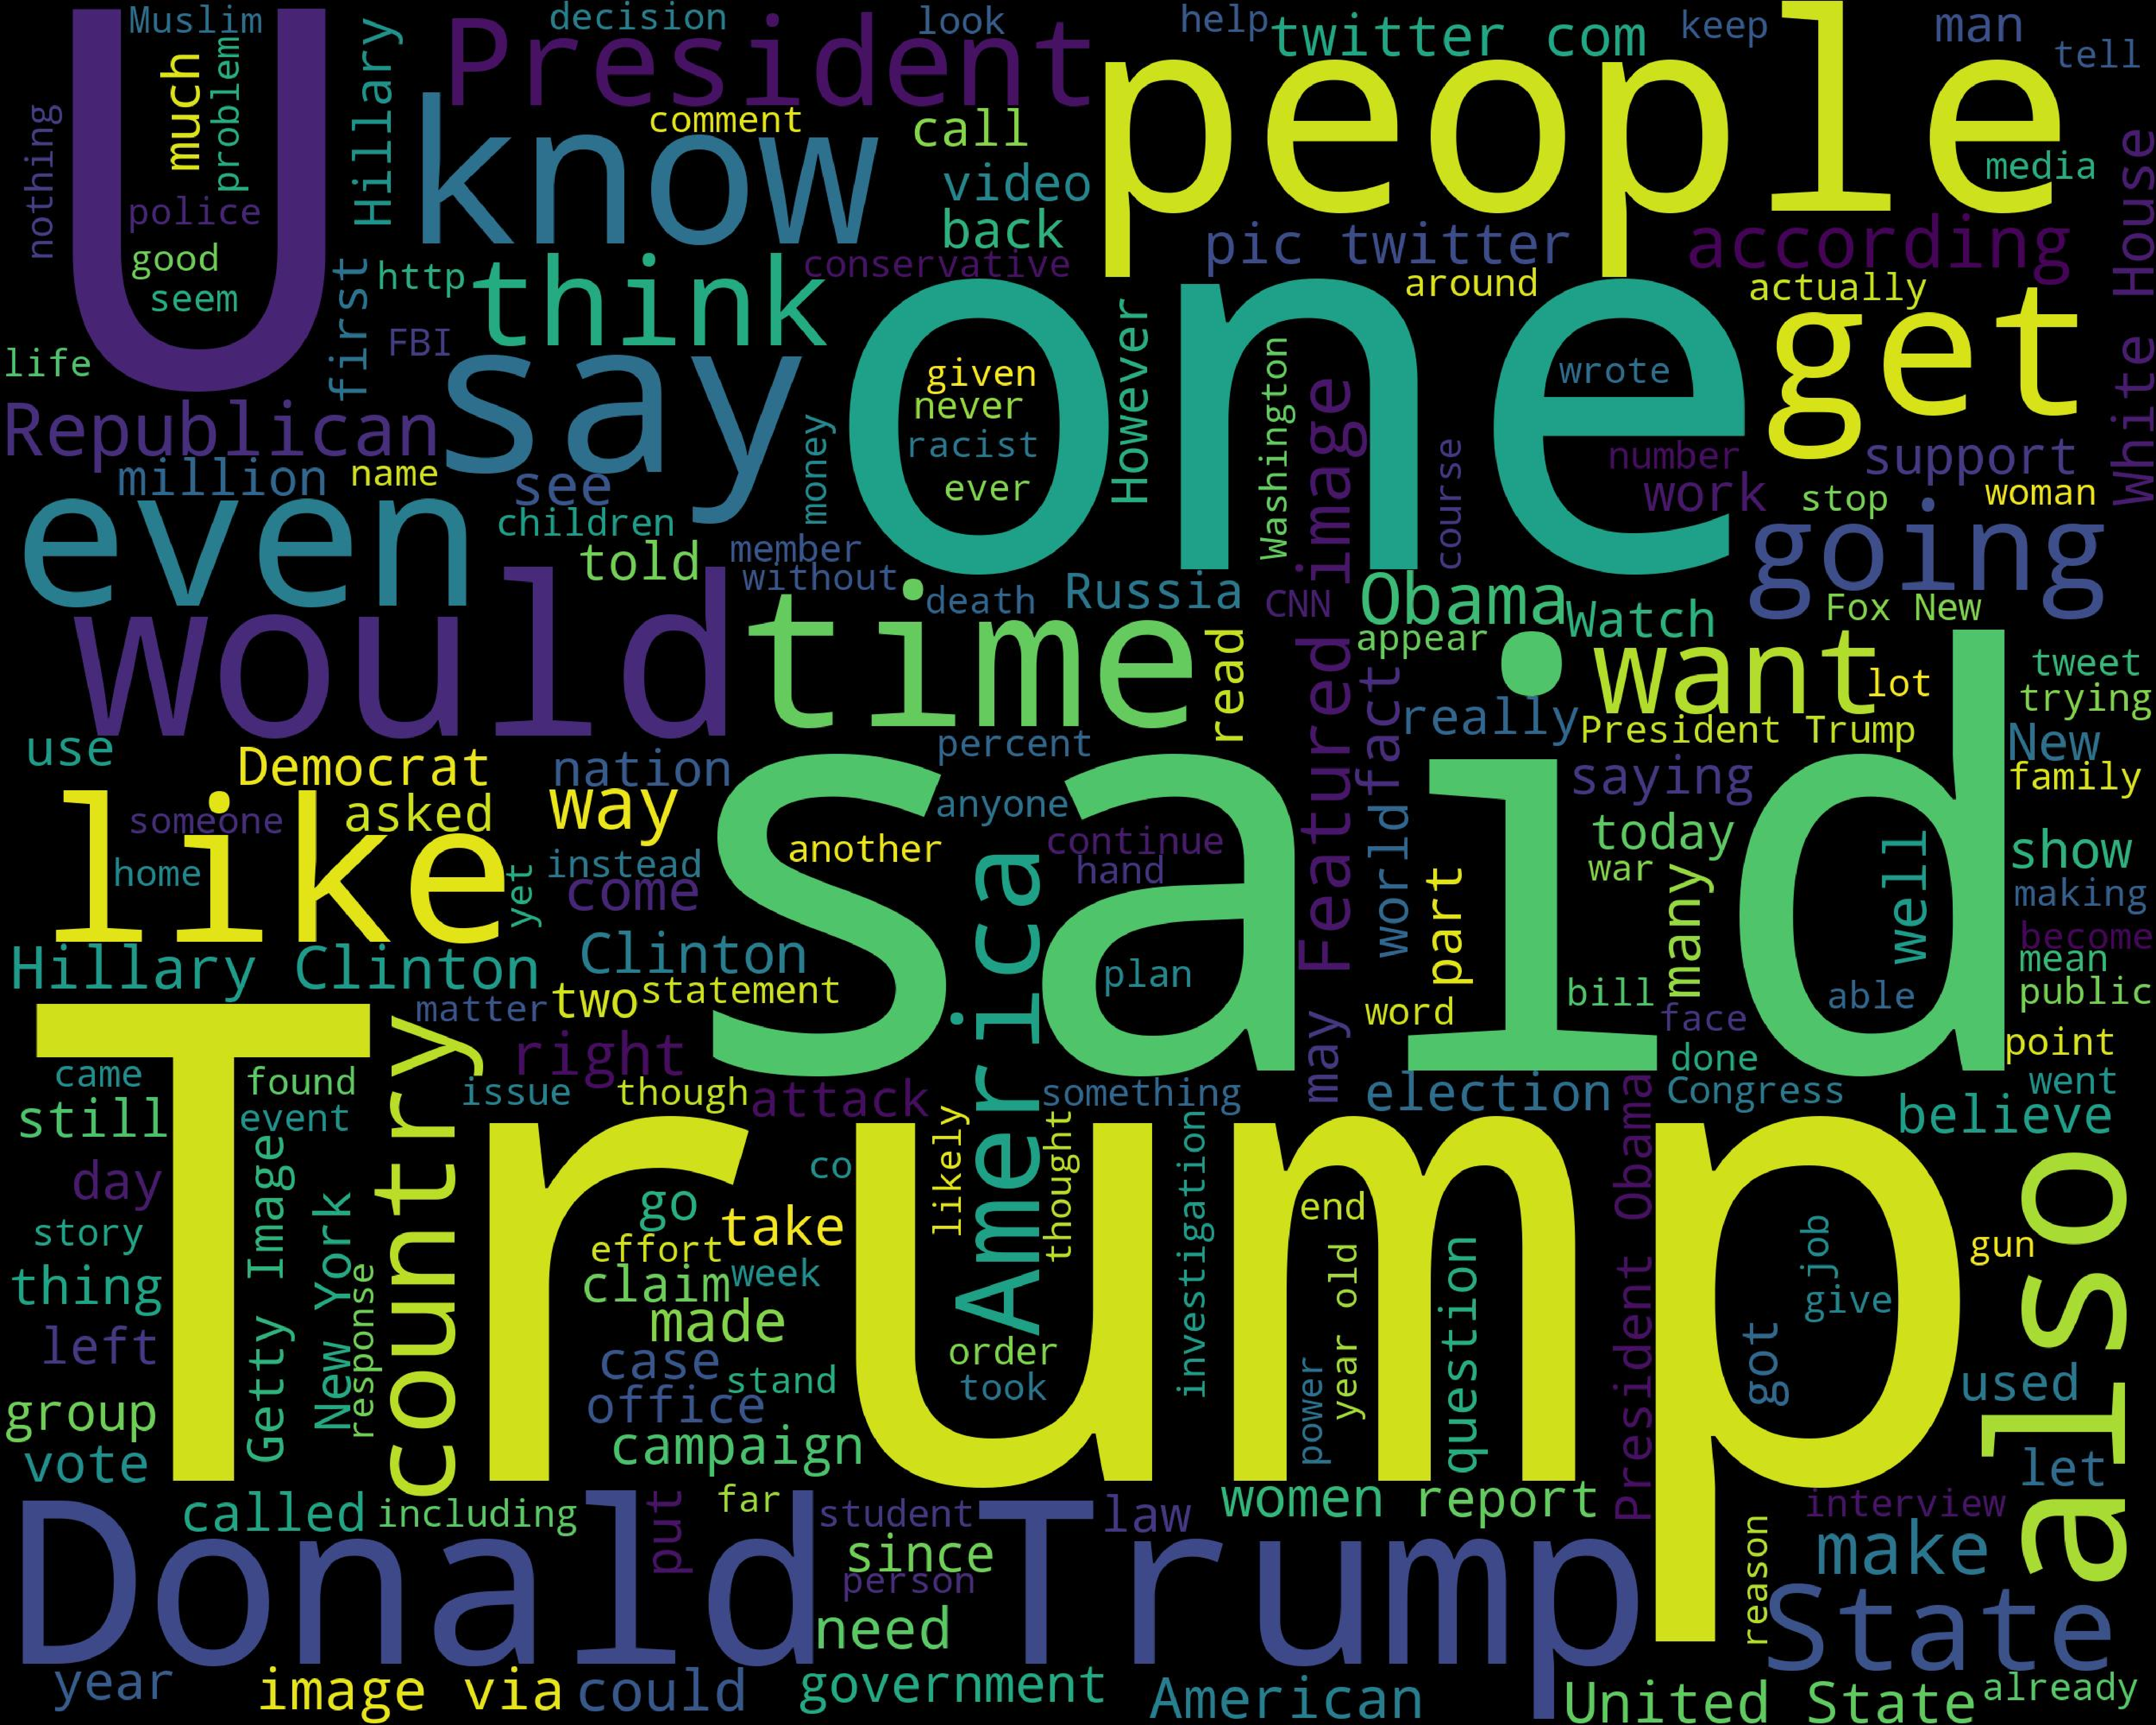
\includegraphics[width=0.75\linewidth]{figures/fakenews_wordcloud.pdf}
    \caption{Fake News - word Cloud}
    \label{fig:enter-label}
\end{figure}


 
\subsubsection{{Data Preprocessing}}
 In the text preprocessing phase, several operations are conducted to refine the dataset for subsequent analysis. Initially, class labels are assigned to distinguish between real and fake news articles, with real articles labeled as class 1 and fake articles as class 0. Next, the title and text content of each article are combined into a single cohesive body to streamline the text processing pipeline. This consolidation enhances the effectiveness of subsequent natural language processing (NLP) tasks by providing a unified textual representation for analysis.

Furthermore, certain attributes that do not contribute significantly to the analysis are removed from the dataset. Specifically, the subject field, which differs between real and fake articles, is dropped, along with the date, title, and publisher information for real articles. This pruning of extraneous attributes streamlines the dataset and focuses attention on the essential text content and class labels. Finally, the processed real and fake datasets are merged into a single dataframe, enabling comprehensive analysis and modeling of the combined dataset. The resultant dataframe, denoted as 'df,' encapsulates the consolidated dataset, ready for further exploration and modeling.

\subsubsection{{Feature Engineering}}
In the feature engineering process, the raw text data is preprocessed and transformed into numerical representations suitable for training machine learning models. Initially, the text is tokenized and cleaned to remove punctuation, stopwords, and other irrelevant characters using the NLTK library. This preprocessing step ensures that the text data is in a standardized format and free from noise that could potentially interfere with the learning process. Subsequently, Word2Vec embeddings are generated using the Gensim library, which learns distributed representations of words by capturing their semantic and syntactic relationships. These word embeddings encode rich semantic information and enable the modeling of word context, similarity, and association within the textual data.

Furthermore, the tokenized text sequences are converted into numerical sequences using a tokenizer, where each word is mapped to a unique numerical identifier. These numerical representations facilitate the input of text data into deep learning models such as recurrent neural networks (RNNs) or convolutional neural networks (CNNs). To ensure uniform input dimensions, the text sequences are padded or truncated to a fixed length, allowing for efficient processing within the neural network architecture. By transforming the raw text into numerical sequences and embedding them into a continuous vector space, the feature engineering phase lays the groundwork for training robust machine learning models capable of capturing intricate patterns and relationships within the textual data.

\subsubsection{Model Selection}

The chosen neural network architecture for this research project integrates an embedding layer initialized with pre-trained Word2Vec embeddings, followed by an LSTM layer and a dense layer for binary classification. By leveraging pre-trained embeddings, the model can effectively capture semantic information and contextual relationships within the news articles. This initialization ensures that words with similar meanings are represented closer in the embedding space, facilitating the model's ability to understand the underlying semantics of the text. Subsequently, the LSTM layer is incorporated to handle the sequential nature of the input data, enabling the model to capture temporal dependencies and long-term patterns within the text. LSTM networks are particularly well-suited for processing sequential data and have demonstrated effectiveness in various NLP tasks, making them a suitable choice for this classification task.

The addition of a dense layer with a sigmoid activation function allows the model to perform binary classification, predicting the likelihood of a news article being real or fake. By outputting a probability score between 0 and 1, the model can effectively differentiate between the two classes. The binary cross-entropy loss function is employed to optimize the model parameters during training, while accuracy serves as the evaluation metric to assess the model's performance. This architecture strikes a balance between capturing semantic relationships, modeling sequential data, and performing binary classification, thereby demonstrating its efficacy in classifying news articles while considering the complex linguistic structure and contextual nuances present in the text data.


\subsubsection{Model Training and Evaluation}
The dataset was split into training and testing sets using the train test split function, with a default ratio of 75\% for training and 25\% for testing. The model was then trained on the training data for a total of 7 epochs, during which the neural network's parameters were adjusted iteratively to minimize the loss between the predicted and actual class labels. The training process involved monitoring the model's performance on a validation subset, comprising 30\% of the training data, to prevent overfitting and ensure generalization.

    \chapter{Results}
\label{ch:results}
The results chapter tells a reader about your findings based on the methodology you have used to solve the investigated problem. For example: 
\begin{itemize}
    \item If your project aims to develop a software/web application, the results may be the developed software/system/performance of the system, etc., obtained using a relevant methodological approach in software engineering. 
    
    \item If your project aims to implement an algorithm for its analysis, the results may be the performance of the algorithm obtained using a relevant experiment design. 
    
    \item If your project aims to solve some problems/research questions over a collected dataset, the results may be the findings obtained using the applied tools/algorithms/etc. 
\end{itemize}
Arrange your results and findings in a logical sequence. 



\section{A section}

...

\clearpage
\section{Example of a Table in \LaTeX}
Table~\ref{tab:_ex_tab} is an example of a table created using the package \LaTeX  ``booktabs.'' do check the link: \href{https://en.wikibooks.org/wiki/LaTeX/Tables}{wikibooks.org/wiki/LaTeX/Tables} for more details. A table should be clean and readable. Unnecessary horizontal lines and vertical lines in tables make them unreadable and messy. The example in Table~\ref{tab:_ex_tab} uses a minimum number of liens (only necessary ones). Make sure that the top rule and bottom rule (top and bottom horizontal lines) of a table are present. 

\begin{table}[h!]
    \centering
    \caption{Example of a table in \LaTeX}
    \label{tab:_ex_tab}
    \begin{tabular}{llr}     
        \toprule
        \multicolumn{2}{c}{Bike} \\
        \cmidrule(r){1-2}
        Type    &  Color & Price (\pounds) \\
        \midrule
        Electric    & black   & 700   \\
        Hybrid      & blue    & 500   \\
        Road        & blue    & 300   \\
        Mountain    & red     & 300   \\
        Folding     & black   & 500   \\
        \bottomrule
    \end{tabular}
\end{table}

\section{Example of captions style}

\begin{itemize}
    \item The \textbf{caption of a Figure (artwork) goes below} the artwork (Figure/Graphics/illustration). See example artwork in Figure~\ref{fig:chart_a}. 
    \item  The \textbf{caption of a Table goes above} the table. See the example in Table~\ref{tab:_ex_tab}.
    \item  The \textbf{caption of an Algorithm goes above} the algorithm. See the example in Algorithm~\ref{algo:algo_example}.
    \item The \textbf{caption of a Listing goes below} the Listing  (Code snippet). See example listing in Listing~\ref{list:python_code_ex}. 
\end{itemize} 





\section{Summary}
Write a summary of this chapter.




    \chapter{Discussion and Analysis}
\label{ch:evaluation}

Depending on the type of project you are doing, this chapter can be merged with ``Results'' Chapter as `` Results and Discussion'' as suggested by your supervisor. 

In the case of software development and the standalone applications, describe the significance of the obtained results/performance of the system. 



\section{A section}% please use an appropriate section title
Discussion and analysis chapter evaluates and analyses the results. It interprets the obtained results. 



\section{Significance of the findings}
In this chapter, you should also try to discuss the significance of the results and key findings, in order to enhance the reader's understanding of the investigated problem

\section{Limitations} % please discuss limitation of the project 
Discuss the key limitations and potential implications or improvements of the findings.
\section{Summary}
Write a summary of this chapter.
    \chapter{Conclusions and Future Work}
\label{ch:con}
\section{Conclusions}
Typically a conclusions chapter first summarizes the investigated problem and its aims and objectives. It summaries the critical/significant/major findings/results about the aims and objectives that have been obtained by applying the key methods/implementations/experiment set-ups. A conclusions chapter draws a picture/outline of your project's central and the most signification contributions and achievements. 

A good conclusions summary could be approximately 300--500 words long, but this is just a recommendation.

A conclusions chapter followed by an abstract is the last things you write in your project report.

\section{Future work}
This section should refer to Chapter~\ref{ch:results} where the author has reflected their criticality about their own solution. The future work is then sensibly proposed in this section.

\textbf{Guidance on writing future work:} While working on a project, you gain experience and learn the potential of your project and its future works. Discuss the future work of the project in technical terms. This has to be based on what has not been yet achieved in comparison to what you had initially planned and what you have learned from the project. Describe to a reader what future work(s) can be started from the things you have completed. This includes identifying what has not been achieved and what could be achieved. 



A good future work summary could be approximately 300--500 words long, but this is just a recommendation.
    \chapter{Reflection}
\label{ch:reflection}
%%%%%%%%%%%%%%%%%%%%%%%%%%%%%%%
%% Please remove/replace text below
%%%%%%%%%%%%%%%%%%%%%%%%%%%%%%%
Engaging in this research project has been an immensely valuable learning experience for me. Beyond just acquiring technical skills like programming in different languages and using LaTeX for report writing, I've gained insights into the intricate process of problem-solving and research inquiry. One significant aspect of my learning journey was the realization of the importance of a systematic approach in tackling complex problems. From identifying the research question to implementing solutions and analyzing results, I learned to adopt a structured methodology, which greatly enhanced the efficiency and effectiveness of my work.

Throughout the project, I encountered various challenges, some of which I successfully navigated, while others posed significant hurdles. One notable challenge was the need to balance model complexity with computational resources and time constraints. Despite my efforts, I found it challenging to optimize certain aspects of the models without sacrificing performance or exceeding computational limitations. This experience highlighted the importance of careful planning and resource management in research endeavors.

Reflecting on the project, if faced with a similar problem in the future, I would approach it with a more robust plan for handling computational constraints and optimizing model architectures. Additionally, I would prioritize more comprehensive data exploration and feature engineering to extract maximum insights from the dataset. Rationalizing the deviations from my initial aims and objectives, I recognize that the dynamic nature of research often necessitates adjustments in approach and priorities. While my overarching goals remained consistent, the iterative nature of the research process led to refinements in methodologies and strategies along the way.

In essence, this research project has equipped me with not only technical skills but also invaluable lessons in research methodology, problem-solving, and project management. Moving forward, I aim to apply these insights to future projects, continually refining my approach and striving for innovation and excellence in my work.
    

    
    % -------------------------------------------------------------------
    % Bibliography/References  -  Harvard Style was used in this report
    % -------------------------------------------------------------------
    \bibliographystyle{agsm} % Harvard Style 
    
    \bibliography{references}  %  Patashnik, O. (1988), BibTEXing. Documentation for general BibTEX users.
    
    % -------------------------------------------------------------------
    % Appendices
    % -------------------------------------------------------------------
    
    \begin{appendices}
        \chapter{An Appendix Chapter (Optional)}
\label{appn:A}
% Optional chapter
Some lengthy tables, codes, raw data, length proofs, etc. which are \textbf{very important but not essential part} of the project report goes into an Appendix. An appendix is something a reader would consult if he/she needs extra information and a more comprehensive understating of the report. Also, note that you should use one appendix for one idea.

An appendix is optional. If you feel you do not need to include an appendix in your report, avoid including it. Sometime including irrelevant and unnecessary materials in the Appendices may unreasonably increase the total number of pages in your report and distract the reader.


        \chapter{An Appendix Chapter (Optional)}
\label{appn:B}

...
    \end{appendices}
    
\end{document}
